% -*- root: ../EstadisticaII.tex -*-
\chapter{Clasificación}


Disponemos de una muestra de $k$ variables medidas en $n$ unidades u objetos que pertenecen a dos grupos o poblaciones \textit{(training data)}.

Cada observación $i=1,\ldots,n$ consiste en un vector $(x'_i,y_i)'$, donde $x_i\in\mathbb{R}^k$ son las $k$ variables e    $y\in\{0,1\}$ indica el grupo al que pertenece la unidad en la que se han obtenido. 

\textbf{Objetivo:} Asignar una nueva unidad con valores $x$ (e $y$ desconocida) a uno de los dos grupos (\textbf{obtener una regla de clasificación}).


Este problema tiene diferentes nombres en la literatura en inglés: ``supervised classification", ``statistical learning", ``discrimination", ``machine learning", ``pattern recognition", etc.

Vamos a ver un ejemplo, para entender mejor el tema

\begin{example}
En un estudio de factores de riesgo en enfermedades coronarias, se dispone de datos de 462 personas (de las que 160 habían sufrido infartos y 302 eran controles). Para cada una de ellas se midieron las siguientes variables:


\begin{center}
\label{example:infartos}
{\scriptsize

\begin{tabular}{|c|l|}
\hline Nombre variable & Descripci\'{o}n  \\
\hline {\tt sbp} & Tensión sanguínea sistólica \\
{\tt tobacco} & Consumo de tabaco\\
{\tt ldl} & Colesterol\\
{\tt adiposity} & Medida de adiposidad\\
{\tt typea} & Comportamiento ``tipo A"\\
{\tt obesity} & Medida de la obesidad\\
{\tt alcohol} & Consumo de alcohol\\
{\tt age} & Edad \\
 \hline
 \end{tabular}

 }
\end{center}

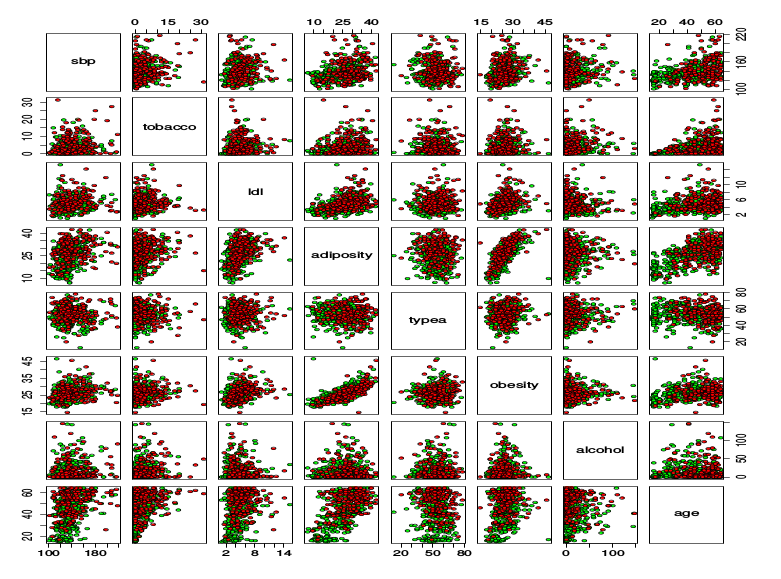
\includegraphics[scale=0.5]{img/pairs-heart.png}


Ahora nos gustaría poder predecir si un nuevo individuo va a tener un infarto o no en función de su consumo de tabaco, colesterol, ...
\end{example}


\section{Regla de Mahalanobis}

La idea es asignar el nuevo individuo al grupo cuyo centro es más cercano (cercano en el sentido de la distancia de Mahalanobis).


\begin{defn}[Regla\IS de Mahalanobis]
Para $i=0,1$ denotamos $P_i$  a la distribución condicionada  $X|Y=i$. Suponemos que $P_i$ es una distribución con vector de medias $\mu_i$ y matriz de covarianzas $\Sigma_i$.


\textbf{Regla de Mahalanobis:} Clasificar $x$ en el grupo 1 (i.e. $Y=1$) si y solo si
\[
(x-\mu_0)'\Sigma_0^{-1}(x-\mu_0) >  (x-\mu_1)'\Sigma_1^{-1}(x-\mu_1).
\]
\end{defn}
En la práctica se usan los vectores de medias y las matrices de covarianzas muestrales, ya que no disponemos de los reales.

La frontera de clasificación sería cuando 
\[
(x-\mu_0)'\Sigma_0^{-1}(x-\mu_0) =  (x-\mu_1)'\Sigma_1^{-1}(x-\mu_1).
\]

Esta frontera será una curva cuadrática (por ser una igualdad entre formas cuadráticas). 

\begin{example}


\centerline{$\mu_0=(1,0)^\prime$, $\mu_1=
(5,0)^\prime$, $\Sigma_1=\left[
  \begin{array}{cc}
    1 & 0 \\
    0 & 1 \
  \end{array} \right]$,
$\Sigma_2=\left[
  \begin{array}{cc}
    5 & 0 \\
    0 & 5 \
  \end{array} \right]$.}

\begin{center}
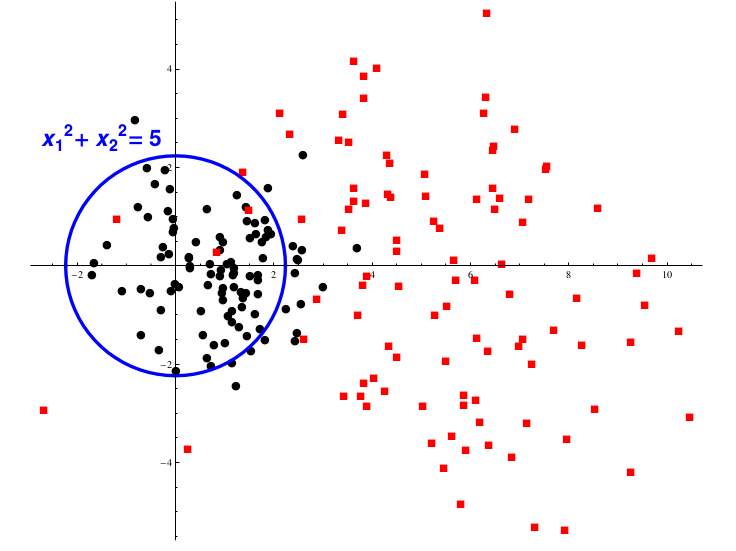
\includegraphics[width=11cm]{img/ReglaMahalanobis.png}
\end{center}

\end{example}

\section{Regla de Fisher}

Vamos a suponer $Σ_1 = Σ_0$, que es cuando mejor funciona esta regla. Vamos a suponer que tenemos estos datos:

\begin{center}
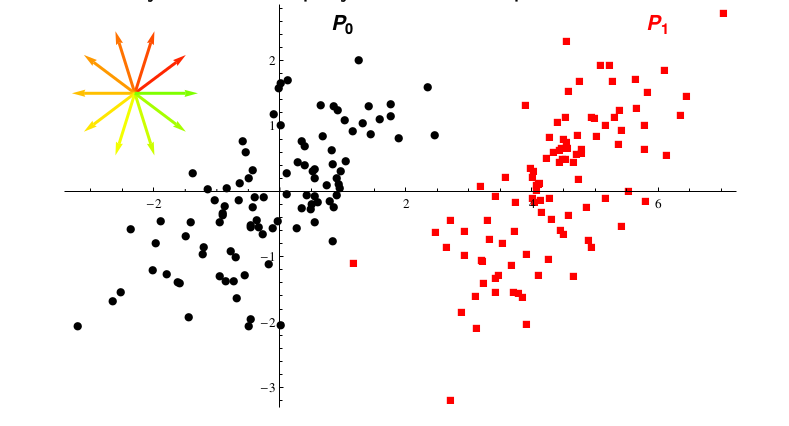
\includegraphics[width=11cm]{img/ReglaFisherIntro.png}
\end{center}


Y la idea intuitiva es construir una recta sobre la que proyectar, para construir 2 histogramas. Si nos dan un nuevo dato, lo clasificaremos en el histograma al que sea más probable que pertenezca.

\begin{center}
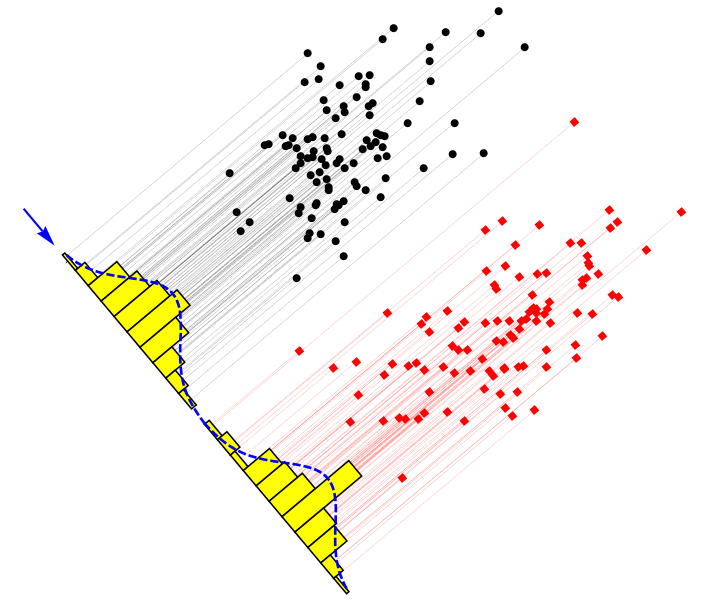
\includegraphics[width=11cm]{img/ReglaFisherIntuitiva.png}
\end{center}


\paragraph{¿Cómo construir esta recta?} Tenemos que tener en cuenta 2 cosas:


\begin{itemize}
  \item Una buena direcci\'{o}n debe separar bien los centros de los grupos. La distancia entre las medias $(a'\mu_0-a'\mu_1)^2 = a'Ba$, donde $B=(\mu_0-\mu_1)(\mu_0-\mu_1)'$, debe ser grande.

\centerline{{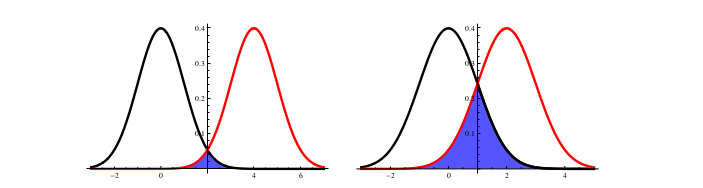
\includegraphics[width=11 cm]{img/FisherNormales.png}}}

  \item La varianza de las proyecciones dentro de los grupos ($a'\Sigma a$) debe ser lo menor
  posible.

\centerline{{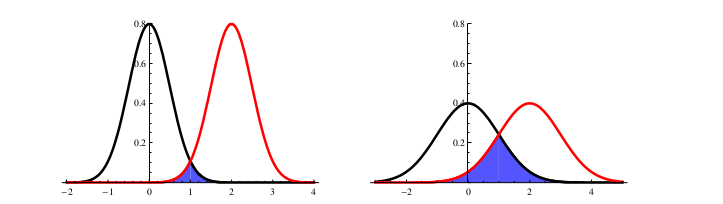
\includegraphics[width=11 cm]{img/FisherNormales2.png}}}

\end{itemize}


La idea de Fisher fue maximizar el ratio de la separación de los centros entre las varianzas, es decir, maximizar el \concept{Cociente\IS de Rayleigh}

\[
f(a) = \frac{a'Ba}{a'\Sigma a} 
\]

para cualquier dirección $a∈ℝ^n$.

\obs Este problema tiene infinitas soluciones, ya que $f(a) = f(λa) ∀λ∈ℝ$. Para solucionar esto, imponemos la normalización tal que $a'Σa = 1$ (aunque no sea la única).

Vamos a calcular el máximo de esta función\footnote{Utilizamos $\grad a'Σa = 2aΣ$. La derivada de una forma cuadrática que es algo que ya deberíamos haber sabido de otras asignaturas del grado.}

\[
\grad f(a) = \frac{2Ba(a'Σa) - 2Σa(a'Ba)}{(a'Σa)^2} \to \grad f(ω) = 0 \dimplies Bω(ω'Σω) = Σω(ω'Bω)
\]

Si llegamos a encontrar ese $ω$, tendrá estas 2 propiedades
\begin{itemize}
	\item $Bω = (µ_0-µ_1)\underbrace{(µ_0 - µ_1)'ω}_{α}$ siendo $α$ un escalar. Esto quiere decir que $Bω = (µ_0-µ_1)α$, esto es: $Bω$ es proporcional a $µ_0 - µ_1$. 
	\item $Σω$ es proporcional a $Σ^{-1}(µ_0 - µ_1)$
\end{itemize}

\begin{defn}[Regla\IS de Fisher] Clasificar $x$ en el grupo 1 (i.e. $Y=1$) si y solo si
\[
ω'\left(x-\frac{\mu_0 + \mu_1}{2}\right)>0
\]
donde $ω=\Sigma^{-1}(\mu_1-\mu_0).$

En caso de tener $ω'\left(x-\frac{\mu_0 + \mu_1}{2}\right)<0$, clasificaríamos en el grupo 2.
\end{defn}


\section{Regresión logística}